\documentclass{article}

\usepackage[english]{babel}

\usepackage[letterpaper,top=1cm,bottom=1cm,left=2cm,right=2cm,marginparwidth=1.75cm]{geometry}

\usepackage{amsmath}
\usepackage{tikz}
\usepackage{multicol}
\usepackage{siunitx}
\usetikzlibrary{intersections, arrows.meta}
\usepackage[colorlinks=true, allcolors=blue]{hyperref}

\title{Normal Force Analyses}
\author{Cole Kauder-McMurrich}
\date{\today}

\begin{document}
% \maketitle

\newcommand*\circled[1]{\tikz[baseline=(char.base)]{
            \node[shape=circle,draw,inner sep=2pt] (char) {#1};}}


            \newcommand*\mss{\unit{m/s^2}}

            \newcommand*\VecUnit[2]{\unit{#1}[#2]}

            \center{\section*{Going down}}
\begin{multicols}{2}

    \center{\underline{\circled{1} {Givens}}}

    \begin{equation*}
        \begin{aligned}
            &m=66.678 \unit{kg}\\
            &\vec{g}=9.81\unit{m/s^2}[D]\\
            &\vec{a}_{su}=0.8 \unit{m/s^2}[D]\\
            &\vec{a}_{sd}=0.3 \unit{m/s^2}[U]\\
        \end{aligned}
    \end{equation*}
    \hfill

    \center{\underline{\circled{2} {Rearrange}}}
    \begin{equation*}
        \begin{aligned}
            \Sigma \vec{F} &= \vec{F}_{net}\\
            \vec{F}_{net} &= \vec{F}_{g} + \vec{F}_{n}\\
            \vec{F}_{g} + \vec{F}_{n} &= m \vec{a}\\ 
            \vec{F}_{n} &= m \vec{a} - \vec{F}_g\\
            \vec{F}_{n} &= m \vec{a} - m \vec{g}\\
        \end{aligned}
    \end{equation*}

    \columnbreak

    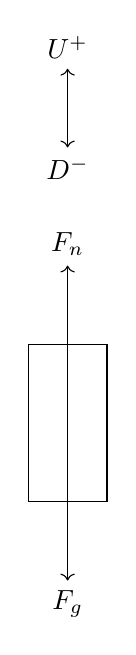
\begin{tikzpicture}
        \draw[<->] (0,3.5) coordinate (down) -- (0, 4.5) coordinate (up);
    
        \node at (up)[anchor=south] {$U^+$};
        \node at (down)[anchor=north] {$D^-$};

        \draw (-0.5, -1) rectangle (0.5, 1);

        \draw[->] (0, 0) -- ++ (0, 2) node [anchor=south]{$F_n$};
        \draw[->] (0, 0) -- ++ (0, -2) node [anchor=north]{$F_g$};
    \end{tikzpicture}

\end{multicols}

\begin{multicols}{2}

    \center{\underline{\circled{3} {Solve for speeding up}}}
    \begin{equation*}
        \begin{aligned}
            \vec{F}_{n} &= m \vec{a}_{su} - m \vec{g}\\
            \vec{F}_{n} &= (66.678 \unit{kg}) (-0.8\mss) - (66.68 \unit{kg})(-9.81\mss)\\
            \vec{F}_{n} &= (66.678 \unit{kg}) (-0.8\mss) -  (-654.13 \unit{N})\\
            \vec{F}_{n} &= (-53.342 \unit{N}) - (-654.13 \unit{N})\\
            \vec{F}_{n} &= 600.7876 \unit{N}
        \end{aligned}
    \end{equation*}

    \fbox {$\vec{F}_{n} = 600.7876 \VecUnit{N}{U}$}

    \center{\underline{\circled{4} {Solve for slowing down}}}
    \begin{equation*}
        \begin{aligned}
            \vec{F}_{n} &= m \vec{a}_{sd} - m \vec{g}\\
            \vec{F}_{n} &= (66.678 \unit{kg}) (0.3\mss) - (66.68 \unit{kg})(-9.81\mss)\\
            \vec{F}_{n} &= (66.678 \unit{kg}) (0.3\mss) - (-654.13 \unit{N})\\
            \vec{F}_{n} &= 20.003 \unit{N} - (-654.13 \unit{N})\\
            \vec{F}_{n} &= 674.133 \unit{N}
        \end{aligned}
    \end{equation*}
    \fbox {$\vec{F}_{n} = 674.133 \VecUnit{N}{U} $}

\end{multicols}

\end{document}

